% !TEX program = xelatex
% Статья: Сплайновая модель траектории камеры для генерации синтетических
% инерциальных измерений в задачах визуально-инерциальной навигации.
% Сборка: tectonic -o build article.tex  (или make article)

\documentclass{misisarticle}

\usepackage{tikz}
\usetikzlibrary{arrows.meta}
\usepackage{pgfplots}
\pgfplotsset{compat=1.18}

% --- Обозначения ---
\newcommand{\Exp}{\operatorname{Exp}}
\newcommand{\Log}{\operatorname{Log}}
\newcommand{\cross}[1]{[#1]_{\times}}
\newcommand{\R}{\mathbb{R}}
\newcommand{\SO}{\mathrm{SO}(3)}
\newcommand{\T}{^{\mathsf{T}}}
\newcommand{\vb}[1]{\mathbf{#1}}

% --- Классификационные коды ---
\grnti{27.41.17, 28.17.19}
\asjc{2605, 2612}
\oecd{1.1}

% --- Название ---
\title{Сплайновая модель траектории камеры для генерации синтетических инерциальных измерений в задачах визуально-инерциальной навигации}

% --- Авторы ---
\misisauthor{К.~И.~Егорова}{кафедра инженерной кибернетики НИТУ «МИСИС»}{Москва, Россия}{m2304019@edu.misis.ru}
\misisauthor{В.~В.~Семёнов}{кафедра инженерной кибернетики НИТУ «МИСИС»}{Москва, Россия}{semenov.vv@misis.ru}

% --- Аннотация и ключевые слова ---
\abstract{%
  Рассматривается генерация синтетических показаний инерциального измерительного блока (IMU) по заданной траектории камеры для тестирования алгоритмов визуально-инерциальной навигации. При задании движения отрезками прямых и сферической линейной интерполяцией поворотов скорость и угловая скорость в узлах меняются скачком, а ускорение содержит импульсы. Формализовано условие согласованности: для траекторий с непрерывной скоростью, дважды непрерывно дифференцируемых на кусках разбиения, идеальные (без шума) показания IMU непрерывны при любом взаимном расположении камеры и IMU тогда и только тогда, когда положение и ориентация камеры принадлежат классу $C^2$. Положение представлено кубическим B-сплайном, ориентация~--- кумулятивным кубическим B-сплайном на группе $\SO$; производные вычисляются по замкнутым формулам. Для проверки модели предложено обратное интегрирование измерений с оценкой наблюдаемого порядка сходимости. В вычислительном эксперименте наблюдаемый порядок по ошибке положения равен 0 для кусочно-линейной модели, 1 для модели со SQUAD и 2 для B-сплайнов при отсчётах, не связанных с узлами (4~--- при отсчётах в узлах). При отсчётах, сдвинутых относительно узлов, он совпадает с оценкой $\min(4, m+1)$, где $m$~--- номер разрывной производной, и для положения, и для ориентации. Шумовая часть генератора проверена по вариации Аллана.
}

\keywords{%
  визуально-инерциальная навигация, SLAM, инерциальный измерительный блок (IMU), B-сплайн, группа вращений SO(3), сплайн-интерполяция, синтетические данные
}

\begin{document}

\maketitle

% ============================================================
\section{Введение}

Визуально-инерциальная навигация (VIO) и визуально-инерциальный SLAM оценивают движение камеры по изображениям и показаниям инерциального измерительного блока (IMU), состоящего из трёхосевого акселерометра и трёхосевого гироскопа. Такие системы, например VINS-Mono~\cite{vinsmono}, ORB-SLAM3~\cite{orbslam3} и OpenVINS~\cite{openvins}, применяются на мобильных роботах и беспилотных летательных аппаратах. Для их сравнения и отладки нужны наборы данных с известной эталонной траекторией.

Наборы EuRoC~\cite{euroc} и TUM VI~\cite{tumvi} записаны на реальных платформах; эталон в них получен внешней системой: захвата движения или, в части записей EuRoC, лазерным трекером, измеряющим только положение. Эталон доступен только в зоне действия такой системы, сам содержит погрешность, а параметры эксперимента (характер движения, уровень шума датчиков, взаимное расположение камеры и IMU) зафиксированы и не варьируются независимо. В синтетических данных траектория задаётся программно и известна точно, а параметры можно менять по отдельности.

Синтетические показания пригодны для тестирования, если они согласованы с заданным движением. Акселерометр измеряет удельную силу $R\T(\ddot{\vb p}-\vb g)$, в которую входит вторая производная положения; гироскоп измеряет угловую скорость, которая выражается через первую производную ориентации: $\cross{\boldsymbol\omega}=R\T\dot R$~\cite{woodman}. Поэтому модель траектории должна обладать достаточным числом непрерывных производных. При задании движения отрезками прямых и сферической линейной интерполяцией ориентаций (SLERP~\cite{shoemake}) скорость и угловая скорость в узлах меняются скачком, ускорение внутри отрезков равно нулю, а в узлах содержит импульсы. Эти скачки вызваны не движением, а способом его задания.

Новый алгоритм навигации в работе не предлагается. Вклад работы:
\begin{itemize}
  \item формализовано условие согласованности модели движения и показаний IMU при смещённой камере: принадлежность классу $C^2$ и положения, и ориентации камеры необходима и достаточна для непрерывности идеальных показаний при любом смещении (утверждение~1);
  \item описан генератор синтетических измерений IMU на основе кубических B-сплайнов в $\R^3$ и на $\SO$ с замкнутыми выражениями для производных и проверкой гладкости на стыках отрезков;
  \item предложена и проверена в вычислительном эксперименте методика, в которой наблюдаемый порядок сходимости обратного интегрирования служит численной мерой гладкости модели движения.
\end{itemize}

Работа является частью выпускной квалификационной работы, посвящённой генерации синтетических визуально-инерциальных данных. Построенная траектория используется также для рендеринга изображений сцены, реконструированной методом гауссова сплаттинга~\cite{kerbl}; изображения и показания IMU вычисляются по одной непрерывной траектории и потому согласованы по времени и движению. Этим определяется выбор системы, для которой задаётся сплайн. Если задать сплайн для камеры, отрендеренную последовательность кадров можно использовать повторно с разными внешними калибровками камера--IMU: меняются только показания IMU, и повторный рендер не нужен. Если сплайн задан для IMU, смена калибровки меняет траекторию камеры, и кадры приходится рендерить заново. Плата за выбор камеры~--- необходимость углового ускорения при пересчёте показаний в точку IMU.

% ============================================================
\section{Анализ работ}

\subsection{Наборы данных и оценка траекторий}

Набор EuRoC~\cite{euroc} содержит стереоизображения и показания IMU, записанные на беспилотнике, и эталон от лазерного трекера или системы захвата движения; TUM VI~\cite{tumvi} дополнительно предоставляет фотометрическую калибровку и записи в различных условиях. Метрики абсолютной ошибки траектории (ATE) и относительной ошибки позы (RPE) введены в~\cite{sturm}; их применение к визуально-инерциальным системам, включая выбор способа совмещения оценки с эталоном, разобрано в~\cite{zhang}.

Эталонная траектория требуется и для оценки алгоритмов замыкания цикла в лидарной одометрии~\cite{epifanov}: коррекция накопленного дрейфа оценивается по отклонению от эталона на замкнутых маршрутах. Генератор с программно заданной траекторией позволяет строить такие маршруты с известной геометрией. Методы стереозрения~\cite{ermolenko} восстанавливают трёхмерное облако точек по карте диспаритета. В настоящей работе геометрия сцены восстанавливается гауссовым сплаттингом~\cite{kerbl}, а изображения рендерятся из известных поз камеры; это позволяет получать стереопары с точно известной внешней калибровкой и использовать их для проверки методов, подобных~\cite{ermolenko}.

\subsection{Непрерывные представления траектории}

Для слияния данных датчиков с разной частотой траекторию задают как непрерывную функцию времени. В~\cite{furgale} траектория представлена B-сплайном, что позволило совместно оценивать пространственную калибровку датчиков и смещение их временных шкал (метод реализован в пакете Kalibr). В~\cite{lovegrove, patronperez} траектория представлена кумулятивным кубическим B-сплайном на группе $\mathrm{SE}(3)$; кумулятивный базис для кватернионных кривых построен в~\cite{kim}. Это представление позволяет моделировать камеры со скользящим затвором и вычислять производные, необходимые для сравнения с показаниями IMU. Непрерывное представление используется также в визуально-инерциальной одометрии для событийных камер~\cite{mueggler}. В~\cite{sommer} получены рекуррентные формулы для угловой скорости и углового ускорения кумулятивного B-сплайна на группах Ли со сложностью, линейной по порядку сплайна. Обзор методов интерполяции движения твёрдого тела высших порядков приведён в~\cite{haarbach}.

Генерация показаний инерциальных датчиков по непрерывной модели движения реализована, например, в симуляторе IMUSim~\cite{imusim}. В симуляторе платформы OpenVINS~\cite{openvins} по заданной траектории строится кубический B-сплайн на $\mathrm{SE}(3)$; в комментарии к исходному коду класса сплайна~\cite{ovcode} прямо указано, что кубический сплайн выбран ради непрерывности класса $C^2$, необходимой для вычисления инерциальных измерений. Сплайн там задаёт позу IMU, поэтому пересчёт позы в систему камеры выполняется жёстким преобразованием и углового ускорения не требует. В настоящей работе ключевые позы задаются для камеры (причина указана во введении), поэтому для вычисления ускорения IMU необходимо угловое ускорение камеры (см.~\eqref{eq:accB}), и требование $R\in C^2$ становится существенным.

Выбрана раздельная модель $\R^3\times\SO$, а не сплайн на $\mathrm{SE}(3)$: производные положения в ней являются многочленами по времени, а положение не зависит от способа интерполяции ориентации. Последнее свойство используется при сравнении моделей в подразделе~IV-F.

Требование $C^2$ к траектории IMU для генерации данных известно~\cite{ovcode}. В известных авторам работах не сформулировано явно, что при смещённой камере класса $C^2$ должна быть и ориентация, и не проводится количественное сравнение с более простыми способами интерполяции.

\subsection{Интерполяция ориентаций}

Сферическая линейная интерполяция кватернионов SLERP введена в~\cite{shoemake}; она даёт постоянную угловую скорость на каждом отрезке и её скачки в узлах. Кубическая сферическая интерполяция SQUAD~\cite{shoemake87} строится из вложенных операций SLERP. При равномерной сетке узлов она обеспечивает непрерывность угловой скорости в узлах; непрерывность углового ускорения в общем случае не обеспечивается.

Ограничения на гладкость траектории возникают также в планировании движения. Планировщики для мобильных манипуляторов, учитывающие достижимость~\cite{ly}, строят траектории с кинематическими ограничениями; такие траектории могут служить источником ключевых поз для генератора при выполнении условий раздела~III.

% ============================================================
\section{Постановка задачи}

\subsection{Системы координат и модель измерений}

Используются три правые системы координат (рис.~\ref{fig:frames}): мировая $W$ (ось $z$ направлена вверх), система IMU $B$ и система камеры $C$. Матрица $R_{XY}\in\SO$ переводит координаты вектора из системы $Y$ в систему $X$. Поза IMU задаётся парой $R_{WB}(t)$, $\vb p_{WB}(t)\in\R^3$, поза камеры~--- парой $R_{WC}(t)$, $\vb p_{WC}(t)$; внешняя калибровка~--- постоянными $R_{BC}$, $\vb p_{BC}$. Вращения представляются гамильтоновыми единичными кватернионами с порядком компонент $(w,x,y,z)$, как в EuRoC~\cite{euroc}; соглашения соответствуют~\cite{sola}. Ускорение свободного падения $\vb g_W=(0,0,-9{,}81)\T$~м/с$^2$.

\begin{figure}[htbp]
  \centering
  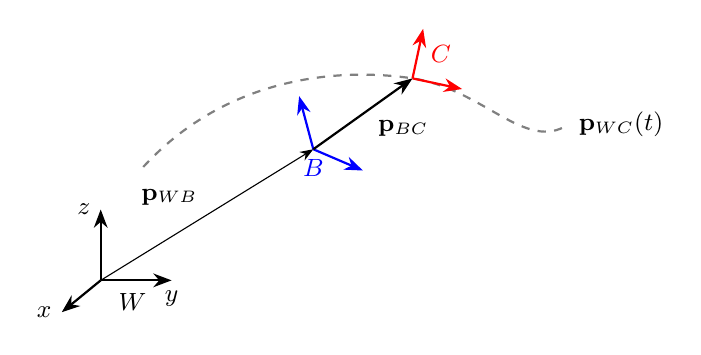
\begin{tikzpicture}[>=Stealth, scale=0.9, every node/.style={font=\small}]
    % мир
    % правая тройка: x -- «на нас», y -- вправо, z -- вверх
    \draw[->, thick] (0,0) -- (1.0,0) node[below] {$y$};
    \draw[->, thick] (0,0) -- (0,1.0) node[left] {$z$};
    \draw[->, thick] (0,0) -- (-0.55,-0.45) node[left] {$x$};
    \node[below] at (0.45,-0.05) {$W$};
    % камера (траектория p_WC проходит через C)
    \coordinate (C) at (4.4,2.85);
    \draw[gray, dashed, thick] (0.6,1.6) .. controls (1.8,2.9) and (3.4,3.0) .. (C)
      .. controls (5.4,2.7) and (6.0,1.8) .. (6.6,2.2)
      node[right, black] {$\vb p_{WC}(t)$};
    % IMU
    \coordinate (B) at (3.0,1.85);
    \draw[->, thick, blue] (B) -- ++(0.7,-0.3);
    \draw[->, thick, blue] (B) -- ++(-0.2,0.75);
    \node[blue, below] at (B) {$B$};
    \draw[->, thick, red] (C) -- ++(0.7,-0.15);
    \draw[->, thick, red] (C) -- ++(0.15,0.7);
    \node[red] at (4.8,3.2) {$C$};
    % рычаг
    \draw[->, thick] (B) -- (C) node[pos=0.55, below right] {$\vb p_{BC}$};
    % радиус-вектор
    \draw[->, thin] (0,0) -- (B) node[midway, above left] {$\vb p_{WB}$};
  \end{tikzpicture}
  \caption{Системы координат: мировая $W$, IMU $B$ и камеры $C$. Камера смещена относительно IMU на вектор $\vb p_{BC}$.}
  \label{fig:frames}
\end{figure}

Угловая скорость в системе $B$ определяется соотношением $\cross{\boldsymbol\omega_B}=R_{WB}\T\dot R_{WB}$, где $\cross{\cdot}$~--- кососимметрическая матрица векторного произведения. Модель измерений гироскопа и акселерометра~\cite{forster, furgale}:
\begin{align}
  \tilde{\boldsymbol\omega}(t) &= \boldsymbol\omega_B(t) + \vb b_g(t) + \boldsymbol\eta_g(t), \label{eq:gyro}\\
  \tilde{\vb a}(t) &= R_{WB}\T(t)\bigl(\ddot{\vb p}_{WB}(t)-\vb g_W\bigr) + \vb b_a(t) + \boldsymbol\eta_a(t). \label{eq:acc}
\end{align}
Здесь $\boldsymbol\eta_g$, $\boldsymbol\eta_a$~--- белый шум с интенсивностями (корнями из спектральной плотности мощности) $\sigma_g$ [рад/(с$\cdot\sqrt{\text{Гц}}$)] и $\sigma_a$ [м/(с$^2\cdot\sqrt{\text{Гц}}$)]. Смещения нулей~--- случайное блуждание: $\dot{\vb b}_g=\boldsymbol\eta_{bg}$, $\dot{\vb b}_a=\boldsymbol\eta_{ba}$ с интенсивностями $\sigma_{bg}$ [рад/(с$^2\cdot\sqrt{\text{Гц}}$)] и $\sigma_{ba}$ [м/(с$^3\cdot\sqrt{\text{Гц}}$)], $\vb b(t_0)=\vb b_0$. Параметры шума определяют по дисперсии Аллана~\cite{ieee952}.

\subsection{Допущения}

\begin{enumerate}
  \item[Д1.] Система $W$ инерциальна по построению генератора, $\vb g_W$ постоянно; вращение Земли ($\approx7{,}3\cdot10^{-5}$~рад/с) и кориолисово ускорение не моделируются. Это систематический эффект, а не шум: за 100~с он даёт ошибку угла порядка $7\cdot10^{-3}$~рад, что сопоставимо с вкладом шума MEMS-гироскопа или больше его. Допущение согласовано с моделями измерений распространённых VIO-систем~\cite{vinsmono, openvins}: в них член с вращением Земли отсутствует; при необходимости оно добавляется к $\boldsymbol\omega_B$ как известный член.
  \item[Д2.] Камера и IMU жёстко связаны, $R_{BC}$ и $\vb p_{BC}$ постоянны и известны точно; погрешность калибровки моделируется отдельно.
  \item[Д3.] Часы камеры и IMU синхронизированы; временно́е смещение~\cite{furgale} вводится как отдельный параметр при необходимости.
  \item[Д4.] IMU идеален в геометрическом смысле: оси ортогональны и совпадают между датчиками, масштабные ошибки, перекос, насыщение и квантование отсутствуют, акселерометр считается точечным. Эти эффекты не влияют на вывод условий гладкости.
  \item[Д5.] Шумы гауссовы и белые, смещения~--- винеровские процессы, компоненты по осям и между датчиками независимы; это стандартная модель~\cite{furgale, forster}.
  \item[Д6.] Модель кинематическая: динамика носителя не учитывается, $\vb p(t)$ и $R(t)$ задаются независимо (ограничения см. в разделе~VI).
  \item[Д7.] Узлы сплайна равномерные, соседние контрольные вращения отличаются на угол меньше $\pi$; это обеспечивает однозначность $\Log$.
  \item[Д8.] Затвор камеры глобальный: все строки кадра соответствуют одному моменту времени.
\end{enumerate}

\subsection{Связь движения камеры и IMU}

Ключевые позы задаются для камеры (см. введение). Поза IMU выражается через позу камеры:
\begin{equation}
  R_{WB}=R_{WC}R_{BC}\T,\qquad
  \vb p_{WB}=\vb p_{WC}+R_{WC}\,\vb r,
  \label{eq:lever}
\end{equation}
где $\vb r=-R_{BC}\T\vb p_{BC}$~--- положение IMU в системе камеры. Дважды дифференцируя~\eqref{eq:lever} и учитывая $\ddot R_{WC}=R_{WC}\bigl(\cross{\boldsymbol\alpha_C}+\cross{\boldsymbol\omega_C}^2\bigr)$, получаем
\begin{align}
  \ddot{\vb p}_{WB} &= \ddot{\vb p}_{WC}
     + R_{WC}\bigl(\boldsymbol\alpha_C\times\vb r
     + \boldsymbol\omega_C\times(\boldsymbol\omega_C\times\vb r)\bigr), \label{eq:accB}\\
  \boldsymbol\omega_B &= R_{BC}\,\boldsymbol\omega_C, \label{eq:omegaB}
\end{align}
где $\boldsymbol\omega_C$ и $\boldsymbol\alpha_C=\dot{\boldsymbol\omega}_C$~--- угловая скорость и угловое ускорение камеры в её собственной системе.

\subsection{Условия непрерывности показаний}

Будем называть функцию кусочно-$C^2$ на $[t_0,t_K]$, если существует разбиение $t_0=\tau_0<\tau_1<\dots<\tau_M=t_K$, на каждом отрезке $[\tau_m,\tau_{m+1}]$ которого она принадлежит классу $C^2$ (с односторонними производными на концах).

\textbf{Утверждение 1.} Пусть $\vb p_{WC}\in C^1$, $R_{WC}\in C^0$ и обе функции кусочно-$C^2$. Идеальные показания $\boldsymbol\omega_B(t)$ и $\vb a_B(t)=R_{WB}\T(\ddot{\vb p}_{WB}-\vb g_W)$ непрерывны при любом $\vb r\in\R^3$ тогда и только тогда, когда $\vb p_{WC}\in C^2$ и $R_{WC}\in C^2$.

\textit{Доказательство.} Достаточность следует из~\eqref{eq:accB}, \eqref{eq:omegaB}. Необходимость: из непрерывности $\boldsymbol\omega_B=R_{BC}\boldsymbol\omega_C$ следует непрерывность $\boldsymbol\omega_C$, то есть $R_{WC}\in C^1$. При $\vb r=0$ из непрерывности $\vb a_B$ и $R_{WB}$ следует непрерывность $\ddot{\vb p}_{WC}$. Тогда при любом $\vb r$ непрерывна функция $R_{WC}(\boldsymbol\alpha_C\times\vb r)$, так как член с $\boldsymbol\omega_C$ уже непрерывен. Подставляя $\vb r=\vb e_1,\vb e_2,\vb e_3$, получаем непрерывность $\boldsymbol\alpha_C$, то есть $R_{WC}\in C^2$. $\blacksquare$

Доказательство элементарно. Ценность утверждения~--- в явной формулировке условия для смещённой камеры: в известных авторам работах требование $C^2$ формулируется для траектории самого IMU (см. замечание ниже).

Требование $\vb p_{WC}\in C^1$ существенно. Кусочно-линейная модель (модель А в подразделе~IV-F) ему не удовлетворяет: при скачке скорости $\ddot{\vb p}_{WC}$ содержит $\delta$-функцию, и показания акселерометра не определены как функции времени.

\textit{Замечание.} При фиксированном $\vb r\neq0$ не обязательны ни $R_{WC}\in C^2$, ни $\vb p_{WC}\in C^2$: скачок $\ddot{\vb p}_{WC}$ может компенсироваться скачком $R_{WC}(\boldsymbol\alpha_C\times\vb r)$, а составляющая скачка $\boldsymbol\alpha_C$, параллельная $\vb r$, на показания не влияет. Для фиксированного $\vb r$ точное условие непрерывности~--- $\vb p_{WB}\in C^2$ и $R_{WB}\in C^1$, то есть гладкость траектории самого IMU. Именно оно используется, когда сплайн задан для IMU~\cite{openvins}. Утверждение~1 требует непрерывности при всех $\vb r$, то есть при любой внешней калибровке, и потому даёт условие на траекторию камеры.

\subsection{Формулировка задачи}

\textit{Дано:} ключевые позы камеры $(t_k,R_k,\vb p_k)$, $k=0,\dots,K$, $t_k=t_0+k\Delta t$, $R_k\in\SO$, $\vb p_k\in\R^3$ [м]; скорости камеры на концах интервала $\vb v_0$, $\vb v_K$ [м/с] и угловые скорости $\boldsymbol\omega_0$, $\boldsymbol\omega_K$ [рад/с] (в системе камеры); внешняя калибровка $R_{BC}\in\SO$, $\vb p_{BC}\in\R^3$ [м]; частота IMU $f$ [Гц], $h=1/f$; интенсивности шумов $\sigma_g,\sigma_a,\sigma_{bg},\sigma_{ba}$; начальные смещения $\vb b_g(t_0)$, $\vb b_a(t_0)$.

\textit{Пространства решений:} $S_p$~--- кубические сплайны $[t_0,t_K]\to\R^3$ с равномерными узлами $\tau_j=t_0+j\Delta t$; $S_R$~--- кривые вида~\eqref{eq:rot} с контрольными вращениями $Q_0,\dots,Q_{K+2}\in\SO$, $\|\Log(Q_j\T Q_{j+1})\|<\pi$.

\textit{Задача 1 (траектория).} Найти $\vb p\in S_p$: $\vb p(t_k)=\vb p_k$, $k=0,\dots,K$, $\dot{\vb p}(t_0)=\vb v_0$, $\dot{\vb p}(t_K)=\vb v_K$. Найти $R\in S_R$: $R(t_k)=R_k$, $k=0,\dots,K$, $\boldsymbol\omega_C(t_0)=\boldsymbol\omega_0$, $\boldsymbol\omega_C(t_K)=\boldsymbol\omega_K$. Условия на угловую скорость на концах~--- аналог $\vb v_0$, $\vb v_K$ для положения; с ними число уравнений равно числу параметров $3(K+3)$ (см. подраздел~IV-D).

\textit{Задача 2 (генерация).} Для $s_n=t_0+nh$, $n=0,\dots,N$, $N=\lfloor(t_K-t_0)/h\rfloor$, вычислить реализации случайных последовательностей $(\tilde{\boldsymbol\omega}_n,\tilde{\vb a}_n)$ по~\eqref{eq:gyro}, \eqref{eq:acc}, \eqref{eq:noise}.

\textit{Задача 3 (проверка).} Без шума найти зависимости ошибок восстановления $e_p(h)$, $e_R(h)$ и проверить гипотезу $e=O(h^q)$; проверить, что шумовая часть генератора воспроизводит заданные интенсивности (подраздел~IV-F).

% ============================================================
\section{Описание методов}

Все производные траектории вычисляются по замкнутым формулам~\eqref{eq:pos}, \eqref{eq:omega}, \eqref{eq:alpha}; конечные разности не используются, и погрешность дифференцирования не смешивается с моделируемым шумом датчиков.

\subsection{Положение: кубический B-сплайн}

На отрезке $t\in[t_i,t_{i+1})$ введём $u=(t-t_i)/\Delta t\in[0,1)$. Равномерный кубический B-сплайн с контрольными точками $\vb c_i,\dots,\vb c_{i+3}$ записывается в матричной форме~\cite{patronperez}:
\begin{equation}
  \vb p(u)=C\,M\,\boldsymbol\psi(u),\quad
  \boldsymbol\psi(u)=\begin{pmatrix}1\\u\\u^2\\u^3\end{pmatrix},
  \label{eq:pos}
\end{equation}
где $C=(\vb c_i\;\vb c_{i+1}\;\vb c_{i+2}\;\vb c_{i+3})$ и
\begin{equation*}
  M=\frac16\begin{pmatrix}
    1 & -3 & 3 & -1\\
    4 & 0 & -6 & 3\\
    1 & 3 & 3 & -3\\
    0 & 0 & 0 & 1
  \end{pmatrix}.
\end{equation*}
Производные по времени: $\dot{\vb p}=\Delta t^{-1}C M(0,1,2u,3u^2)\T$, $\ddot{\vb p}=\Delta t^{-2}C M(0,0,2,6u)\T$. Кубический B-сплайн с простыми узлами принадлежит $C^2([t_0,t_K];\R^3)$~\cite{deboor}.

\subsection{Ориентация: кумулятивный B-сплайн на $\SO$}

Экспоненциальное отображение $\Exp:\R^3\to\SO$ задаётся формулой Родрига
\begin{equation*}
  \Exp(\boldsymbol\varphi)=I+\frac{\sin\theta}{\theta}\cross{\boldsymbol\varphi}+\frac{1-\cos\theta}{\theta^2}\cross{\boldsymbol\varphi}^2,\quad \theta=\|\boldsymbol\varphi\|,
\end{equation*}
$\Log$~--- обратное к нему отображение при $\theta<\pi$~\cite{sola}.

Обозначим через $B_j(u)$, $j=0,\dots,3$, компоненты вектора $M\boldsymbol\psi(u)$~--- обычные базисные функции, так что $\vb p(u)=\sum_j B_j(u)\vb c_{i+j}$. Эту сумму можно записать через разности соседних контрольных точек с кумулятивными базисными функциями $\tilde B_j(u)=\sum_{l\ge j}B_l(u)$. Для вращений сложение заменяется умножением, разность~--- логарифмом~\cite{kim, lovegrove}:
\begin{equation}
  R(u)=Q_i\prod_{j=1}^{3}\Exp\bigl(\tilde B_j(u)\,\vb d_j\bigr),\quad
  \vb d_j=\Log\bigl(Q_{i+j-1}\T Q_{i+j}\bigr),
  \label{eq:rot}
\end{equation}
где $Q_i,\dots,Q_{i+3}$~--- контрольные вращения. Кумулятивные базисные функции (рис.~\ref{fig:basis}):
\begin{equation}
  \begin{gathered}
    \tilde B_1=\tfrac16\bigl(5+3u-3u^2+u^3\bigr),\\
    \tilde B_2=\tfrac16\bigl(1+3u+3u^2-2u^3\bigr),\quad
    \tilde B_3=\tfrac16u^3.
  \end{gathered}
  \label{eq:cumbasis}
\end{equation}

\begin{figure}[htbp]
  \centering
  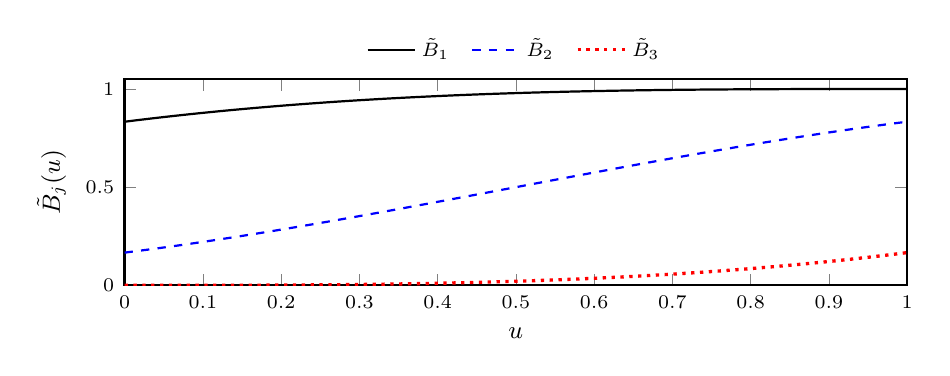
\begin{tikzpicture}
    \begin{axis}[
      width=0.95\columnwidth, height=4.2cm,
      xmin=0, xmax=1, ymin=0, ymax=1.05,
      xlabel={$u$}, ylabel={$\tilde B_j(u)$},
      legend columns=3, legend style={at={(0.5,1.03)}, anchor=south, /tikz/every even column/.append style={column sep=6pt}, font=\scriptsize, draw=none, fill=none},
      tick label style={font=\scriptsize}, label style={font=\small},
      samples=60, domain=0:1, thick]
      \addplot[black] {(5+3*x-3*x^2+x^3)/6};
      \addplot[blue, dashed] {(1+3*x+3*x^2-2*x^3)/6};
      \addplot[red, dotted, very thick] {x^3/6};
      \legend{$\tilde B_1$, $\tilde B_2$, $\tilde B_3$}
    \end{axis}
  \end{tikzpicture}
  \caption{Кумулятивные базисные функции кубического B-сплайна на одном отрезке ($\tilde B_0\equiv 1$).}
  \label{fig:basis}
\end{figure}

Обозначим $A_j=\Exp(\tilde B_j\vb d_j)$ и промежуточные произведения $\Pi_1=Q_i$, $\Pi_{j+1}=\Pi_jA_j$, так что $R(u)=\Pi_4$. Поскольку направление вектора $\tilde B_j\vb d_j$ не зависит от $t$, $A_j\T\dot A_j=\cross{\dot{\tilde B}_j\vb d_j}$. Угловая скорость в собственной системе вычисляется рекуррентно~\cite{sommer}:
\begin{equation}
  \boldsymbol\omega^{(1)}=0,\quad
  \boldsymbol\omega^{(j+1)}=A_j\T\boldsymbol\omega^{(j)}+\dot{\tilde B}_j\vb d_j,
  \label{eq:omega}
\end{equation}
а дифференцирование~\eqref{eq:omega} с учётом $\dot A_j\T=-\cross{\dot{\tilde B}_j\vb d_j}A_j\T$ даёт угловое ускорение:
\begin{equation}
  \boldsymbol\alpha^{(j+1)}=A_j\T\boldsymbol\alpha^{(j)}
  +\bigl(A_j\T\boldsymbol\omega^{(j)}\bigr)\times\dot{\tilde B}_j\vb d_j
  +\ddot{\tilde B}_j\vb d_j,
  \label{eq:alpha}
\end{equation}
где $\boldsymbol\alpha^{(1)}=0$, $\dot{\tilde B}_j=\Delta t^{-1}\,d\tilde B_j/du$, $\ddot{\tilde B}_j=\Delta t^{-2}\,d^2\tilde B_j/du^2$. Искомые величины: $\boldsymbol\omega_C=\boldsymbol\omega^{(4)}$, $\boldsymbol\alpha_C=\boldsymbol\alpha^{(4)}$.

Внутри отрезка функция~\eqref{eq:rot} бесконечно дифференцируема. Гладкость на стыке проверяется непосредственно. Из~\eqref{eq:cumbasis} тройки $(\tilde B_j,\,d\tilde B_j/du,\,d^2\tilde B_j/du^2)$ для $j=1,2,3$ равны
\begin{equation*}
  \begin{aligned}
    u=1&:\ (1,0,0),\ (\tfrac56,\tfrac12,-1),\ (\tfrac16,\tfrac12,1);\\
    u=0&:\ (\tfrac56,\tfrac12,-1),\ (\tfrac16,\tfrac12,1),\ (0,0,0).
  \end{aligned}
\end{equation*}
На отрезке $i$ при $u=1$ первый множитель равен $A_1=\Exp(\vb d_1)$, так что $\Pi_2=Q_i\Exp(\vb d_1)=Q_{i+1}$, а в~\eqref{eq:omega}, \eqref{eq:alpha} он даёт $\boldsymbol\omega^{(2)}=0$, $\boldsymbol\alpha^{(2)}=0$, поскольку $d\tilde B_1/du=d^2\tilde B_1/du^2=0$. Оставшиеся два шага используют тройки $(\tfrac56,\tfrac12,-1)$ и $(\tfrac16,\tfrac12,1)$ с векторами $\vb d_2$, $\vb d_3$. На отрезке $i+1$ при $u=0$ первые два шага начинаются с $\Pi_1=Q_{i+1}$, $\boldsymbol\omega^{(1)}=\boldsymbol\alpha^{(1)}=0$ и используют те же тройки с теми же векторами $\vb d_1'=\vb d_2$, $\vb d_2'=\vb d_3$, а третий шаг тривиален: $A_3=I$, $\dot{\tilde B}_3=\ddot{\tilde B}_3=0$. Следовательно, $R$, $\boldsymbol\omega$ и $\boldsymbol\alpha$ слева и справа от узла совпадают, $R\in C^2([t_0,t_K];\R^{3\times3})$ как функция со значениями в $\R^{3\times3}$, и по утверждению~1 показания IMU непрерывны при любом $\vb r$. Численная проверка (подраздел~V-B) подтверждает совпадение в арифметике с плавающей точкой.

\subsection{Выбор контрольных точек}

При $t=t_i$ (отрезок $i$, $u=0$) условие $\vb p(t_i)=\vb p_i$ принимает вид $(\vb c_i+4\vb c_{i+1}+\vb c_{i+2})/6=\vb p_i$, $i=0,\dots,K$. Краевые условия $\dot{\vb p}(t_0)=(\vb c_2-\vb c_0)/(2\Delta t)=\vb v_0$ и $\dot{\vb p}(t_K)=(\vb c_{K+2}-\vb c_K)/(2\Delta t)=\vb v_K$ позволяют исключить $\vb c_0$ и $\vb c_{K+2}$; первое и последнее уравнения принимают вид $4\vb c_1+2\vb c_2=6\vb p_0+2\Delta t\,\vb v_0$ и $2\vb c_K+4\vb c_{K+1}=6\vb p_K-2\Delta t\,\vb v_K$.

Для ориентации задача~1 нелинейна. Начальное приближение берётся по аналогии с положением: в точке $t_k$ наибольший вес имеет $B_1(0)=2/3$, поэтому
\begin{equation}
  \begin{gathered}
    Q_{k+1}=R_k,\quad k=0,\dots,K;\\
    Q_0=R_0\Exp\bigl(-\Log(R_0\T R_1)\bigr);\\
    Q_{K+2}=R_K\Exp\bigl(\Log(R_{K-1}\T R_K)\bigr).
  \end{gathered}
  \label{eq:qinit}
\end{equation}
Крайние вращения продолжают движение на первом и последнем отрезках; при этом угловое ускорение на концах интервала обращается в нуль, что аналогично естественным краевым условиям сплайна. Приближение~\eqref{eq:qinit} служит начальной точкой. Задача~1 для ориентации решается методом Левенберга--Марквардта по параметрам $\boldsymbol\delta_j$, $Q_j=Q_j^{(0)}\Exp(\boldsymbol\delta_j)$, с вектором невязок $\Log(R_k\T R(t_k))$, $k=0,\dots,K$, и $\Delta t\,(\boldsymbol\omega_C(t_0)-\boldsymbol\omega_0)$, $\Delta t\,(\boldsymbol\omega_C(t_K)-\boldsymbol\omega_K)$. Условия на $\boldsymbol\omega$ на концах снимают асимметрию с положением: угловое ускорение на концах больше не зануляется. Невязки до и после уточнения приведены в подразделе~V-A.

Если позы заданы на неравномерной сетке (например, эталон открытого набора данных), контрольные точки находятся методом наименьших квадратов по всем позам. Шаг $\Delta t$ в этом случае играет роль параметра сглаживания: при слишком крупном шаге высокочастотные составляющие движения не воспроизводятся.

\subsection{Корректность и сложность}

\textit{Положение.} Система из подраздела~IV-C относительно $\vb c_1,\dots,\vb c_{K+1}$ трёхдиагональна со строгим диагональным преобладанием (4 на диагонали; 1 и 1 или 2 рядом), поэтому решение существует, единственно и находится методом прогонки за $O(K)$ операций.

\textit{Ориентация.} Без условий на $\boldsymbol\omega$ на концах система $R(t_k)=R_k$ недоопределена ($K+3$ неизвестных вращения при $K+1$ условиях): матрица Якоби невязок имеет не больше $3(K+1)$ строк при $3(K+3)$ столбцах, и шаг метода Гаусса--Ньютона не определён. Условия на $\boldsymbol\omega$ на концах делают систему квадратной. Она нелинейна, поэтому существование и единственность решения в общем случае здесь не доказываются; метод Левенберга--Марквардта сходится локально, из начальной точки~\eqref{eq:qinit}, удовлетворяющей Д7. Готовая конструкция интерполирующей $C^2$-кривой для кватернионов приведена в~\cite{kim95}.

\textit{Локальность и сложность.} B-сплайн локален: контрольная точка влияет на четыре соседних отрезка. Вычисление одного отсчёта по~\eqref{eq:pos}--\eqref{eq:alpha} требует $O(1)$ операций.

\subsection{Формирование измерений}

В моменты $s_n$ по формулам~\eqref{eq:pos}--\eqref{eq:alpha} вычисляются $R_{WC}$, $\ddot{\vb p}_{WC}$, $\boldsymbol\omega_C$, $\boldsymbol\alpha_C$, по~\eqref{eq:lever}--\eqref{eq:omegaB}~--- кинематика IMU, по~\eqref{eq:gyro}, \eqref{eq:acc}~--- идеальные измерения. Шум и смещения дискретизируются по стандартной схеме~\cite{furgale, forster}:
\begin{equation}
  \begin{gathered}
    \boldsymbol\eta_{g,n}\sim\mathcal N\!\Bigl(0,\tfrac{\sigma_g^2}{h}I\Bigr),\quad
    \boldsymbol\eta_{a,n}\sim\mathcal N\!\Bigl(0,\tfrac{\sigma_a^2}{h}I\Bigr),\\
    \vb b_{n+1}=\vb b_n+\sigma_b\sqrt h\,\boldsymbol\xi_n,\quad
    \boldsymbol\xi_n\sim\mathcal N(0,I),
  \end{gathered}
  \label{eq:noise}
\end{equation}
отдельно для гироскопа ($\sigma_{bg}$) и акселерометра ($\sigma_{ba}$). Параметры берутся из паспорта MEMS-датчика или калибровочных файлов открытых наборов данных~\cite{euroc}. Изображения рендерятся по~\eqref{eq:pos}, \eqref{eq:rot} в моменты кадров.

\subsection{Методика проверки}

\textit{Обратное интегрирование.} Начальное состояние $(\hat R_0,\hat{\vb v}_0,\hat{\vb p}_0)$ системы $B$ берётся из сплайна, после чего траектория восстанавливается по измерениям:
\begin{equation}
  \begin{aligned}
    \hat R_{n+1}&=\hat R_n\Exp\bigl((\tilde{\boldsymbol\omega}_n-\hat{\vb b}_g)h\bigr),\\
    \hat{\vb a}_n&=\hat R_n(\tilde{\vb a}_n-\hat{\vb b}_a)+\vb g_W,\\
    \hat{\vb v}_{n+1}&=\hat{\vb v}_n+\hat{\vb a}_n h,\quad
    \hat{\vb p}_{n+1}=\hat{\vb p}_n+\hat{\vb v}_n h+\tfrac12\hat{\vb a}_n h^2.
  \end{aligned}
  \label{eq:integr}
\end{equation}
Здесь $\hat{\vb b}_g$, $\hat{\vb b}_a$~--- истинные смещения, известные генератору; в серии~1 они нулевые. Схема~\eqref{eq:integr} имеет первый порядок. Используется также классическая схема Рунге--Кутты четвёртого порядка (РК4) для системы $\dot R=R\cross{\tilde{\boldsymbol\omega}-\hat{\vb b}_g}$, $\dot{\vb v}=R(\tilde{\vb a}-\hat{\vb b}_a)+\vb g_W$, $\dot{\vb p}=\vb v$. Ориентация интегрируется как матрица, после каждого шага она проецируется на $\SO$ через сингулярное разложение. РК4 требует измерений в серединах шагов; генератор вычисляет их в любой момент времени, так что фактически используется IMU частоты $2f$. Для проверки модели это допустимо.

\textit{Метрики.} Ошибка положения $e_p(s_n)=\|\hat{\vb p}_n-\vb p_{WB}(s_n)\|$ и ориентации $e_R(s_n)=\|\Log(\hat R_n\T R_{WB}(s_n))\|$ и их среднеквадратичные значения по траектории (аналог ATE~\cite{sturm, zhang}). Совмещение оценки с эталоном не требуется, так как начальное состояние известно точно.

\textit{Серия 1: сходимость без шума} ($\sigma=0$, $\vb b=0$). При точных производных ошибка убывает как $O(h^q)$, где $q$~--- порядок схемы, если правая часть уравнений движения достаточно гладкая на каждом шаге. Если у правой части в узлах разрывна производная номер $m$ ($m=0$~--- скачок самой функции), шаг, внутри которого лежит узел, даёт локальную ошибку $O(h^{m+1})$; узлов конечное число, поэтому ожидается наблюдаемый порядок $\min(q, m+1)$. У кубического сплайна третья производная положения в узлах разрывна. Поэтому эксперимент проводится на двух сетках:
\begin{itemize}
  \item согласованной: $\Delta t/h$~--- целое, $s_0=t_0$, шаги не пересекают узлов;
  \item сдвинутой: $s_0=t_0+\theta h$ с фиксированной долей $\theta=0{,}37$, так что узел при любом $h$ лежит в одной и той же относительной точке шага.
\end{itemize}
Сдвиг, фиксированный в секундах, не годится: при уменьшении $h$ узел попадает в разные точки шага, и наблюдаемый порядок становится неустойчивым. На согласованной сетке разрыв показаний тоже проявляется: значение в самом узле генератор берёт с одной стороны (отрезки полуоткрыты, $[t_i,t_{i+1})$), и последняя стадия шага, заканчивающегося в узле, получает значение с соседнего отрезка. Поэтому для модели Б на согласованной сетке ожидается первый порядок, если в конце шага не брать односторонний предел слева. Таким образом, наблюдаемый порядок сходимости служит численной мерой гладкости модели движения. Тестовая траектория обязательно содержит вращение: при постоянной ориентации и $\vb r=0$ ускорение кусочно-линейно, и порядок не измерить.

\textit{Серия 2: шумовая часть генератора.} Генерируется запись неподвижного датчика (идеальные показания постоянны), по ней строится перекрывающаяся вариация Аллана $\sigma^2(\tau)$~\cite{ieee952}. Интенсивности оцениваются методом наименьших квадратов по модели $\sigma^2(\tau)=N^2/\tau+K^2\tau/3$ и сравниваются с заданными: $N$ соответствует $\sigma_g$ или $\sigma_a$, $K$~--- $\sigma_{bg}$ или $\sigma_{ba}$.

\textit{Серия 3: сравнение моделей}, построенных по одним ключевым позам (табл.~\ref{tab:models}): А~--- кусочно-линейная с SLERP, Б~--- кубический интерполяционный сплайн с SQUAD, В~--- B-сплайны. При одинаковых краевых условиях кубический интерполяционный сплайн и B-сплайн с контрольными точками из подраздела~IV-C~--- одна и та же функция (единственность решения, подраздел~IV-D). Поэтому сравнение моделей Б и В выделяет влияние способа интерполяции ориентации.

\begin{table}[htbp]
  \caption{Свойства моделей движения: А~--- кусочно-линейная с SLERP, Б~--- кубический сплайн с SQUAD, В~--- B-сплайны}
  \label{tab:models}
  \centering
  \small
  \begin{tabular}{lccc}
    \toprule
    \textbf{Свойство} & \textbf{А} & \textbf{Б} & \textbf{В} \\
    \midrule
    Класс $\vb p(t)$ & $C^0$ & $C^2$ & $C^2$ \\
    Класс $R(t)$ & $C^0$ & $C^1$ & $C^2$ \\
    $\boldsymbol\omega_B$ в узлах & скачок & непр. & непр. \\
    $\vb a_B$ в узлах & импульс & скачок$^{*}$ & непр. \\
    $\vb p(t_k)=\vb p_k$ & да & да & да \\
    $R(t_k)=R_k$ & да & да & да$^{**}$ \\
    \bottomrule
  \end{tabular}

  \smallskip
  {\footnotesize Показания идеальные (без шума). $^{*}$При $\vb r\neq0$. $^{**}$После уточнения (IV-C); невязка приведена в подразделе~V-A. <<Непр.>>~--- непрерывна.}
\end{table}


Для модели А результат серии~1 следует из её построения: внутри отрезков $\ddot{\vb p}_{WC}=0$, скачки скорости в узлах акселерометр не регистрирует (при $\vb r\neq0$ добавляется лишь центростремительный член $R_{BC}(\boldsymbol\omega_C\times(\boldsymbol\omega_C\times\vb r))$), и ошибка положения после первого узла растёт линейно со временем при любом $h$. Угловая скорость модели А кусочно постоянна, поэтому на согласованной сетке схема~\eqref{eq:integr} восстанавливает ориентацию точно, а на сдвинутой~--- с ошибкой $O(h)$.

% ============================================================
\section{Результаты}

\subsection{Условия эксперимента}

Ключевые позы камеры заданы в моменты $t_k=0{,}5k$~с, $k=0,\dots,20$ (10~с): $\vb p_k=(2\sin0{,}4t_k,\ 1{,}5\sin0{,}8t_k,\ 1+0{,}3\sin0{,}6t_k)$~м, $R_k=\Exp(\boldsymbol\varphi(t_k))$, $\boldsymbol\varphi=(0{,}15\sin0{,}9t,\ 0{,}2\sin0{,}7t,\ 0{,}6\sin0{,}3t)$~рад; $\vb v_0$, $\vb v_K$ и $\boldsymbol\omega_0$, $\boldsymbol\omega_K$~--- производные тех же функций. Внешняя калибровка: $\vb p_{BC}=(0{,}08;\,0;\,0{,}03)$~м, $R_{BC}$~--- поворот на $10^\circ$ вокруг оси $z$, $\|\vb r\|=8{,}5$~см. Частота IMU $f=50\dots1600$~Гц, сдвиг сетки $\theta=0{,}37$, в серии~1 шум и смещения нулевые. Невязка начального приближения~\eqref{eq:qinit} по ключевым вращениям~--- до $6{,}3\cdot10^{-3}$~рад ($0{,}36^\circ$), по угловой скорости на концах~--- до $0{,}021$~рад/с. Метод Левенберга--Марквардта сошёлся за 12 вычислений невязки; после уточнения невязка по ключевым вращениям не превышает $6\cdot10^{-17}$~рад, то есть равна нулю с машинной точностью. Положение проходит через ключевые точки с той же точностью. Результаты ниже получены для уточнённой модели~В. Код и данные эксперимента: \url{https://github.com/1Bermud/spline-imu-sim}.

\subsection{Показания в узлах}

Для проверки гладкости значения сравнивались по формулам двух соседних отрезков в общем узле: отрезок $i$ при $u=1$ и отрезок $i+1$ при $u=0$. У модели В угловая скорость и угловое ускорение совпали точно (разность равна нулю в арифметике с плавающей точкой), что подтверждает выкладку подраздела~IV-B. У модели Б скачок $\boldsymbol\alpha_C$ достигает $0{,}12$~рад/с$^2$ по модулю вектора (рис.~\ref{fig:alpha}) при значениях $\|\boldsymbol\alpha_C\|$ до $0{,}2$~рад/с$^2$. Через рычаг он даёт ступеньки идеальных показаний акселерометра до $6{,}5$~мм/с$^2$. У модели А в узлах скачет угловая скорость, до $0{,}076$~рад/с.

\begin{figure}[!tb]
  \centering
  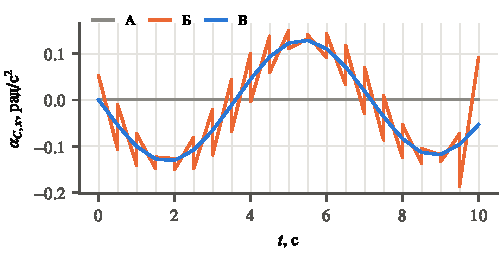
\includegraphics[width=\columnwidth]{figures/alpha.pdf}
  \caption{Угловое ускорение камеры (ось $x$) для моделей А, Б, В. Вертикальные линии~--- узлы. У модели А $\boldsymbol\alpha_C=0$ внутри отрезков; $\delta$-импульсы в узлах не показаны.}
  \label{fig:alpha}
\end{figure}

\subsection{Сходимость обратного интегрирования}

Результаты серии~1 приведены в табл.~\ref{tab:errors} и на рис.~\ref{fig:conv}. Порядок оценивался как наклон прямой, построенной методом наименьших квадратов в логарифмических осях по частотам 100--800~Гц; для модели В на согласованной сетке, где с 400~Гц сказывается округление,~--- по 50--200~Гц.

\begin{table}[!tb]
  \caption{СКО ошибки положения при $f=200$~Гц, м (в скобках~--- наблюдаемый порядок); сетки~--- сдвинутая и согласованная}
  \label{tab:errors}
  \centering
  \small
  \begin{tabular}{lccc}
    \toprule
    & \eqref{eq:integr} & РК4, сдвинутая & РК4, согласованная \\
    \midrule
    А & 8,09 (0) & 8,09 (0) & 8,10 (0) \\
    Б & $9{,}7\cdot10^{-2}$ (1) & $3{,}9\cdot10^{-5}$ (1) & $3{,}2\cdot10^{-5}$ (1)$^{*}$ \\
    В & $1{,}0\cdot10^{-1}$ (1) & $7{,}6\cdot10^{-7}$ (2) & $1{,}1\cdot10^{-11}$ (4) \\
    \bottomrule
  \end{tabular}

  \smallskip
  {\footnotesize $^{*}$С пределом слева в конце шага: $9{,}4\cdot10^{-12}$~м, порядок 3,8.}
\end{table}

\begin{figure}[!tb]
  \centering
  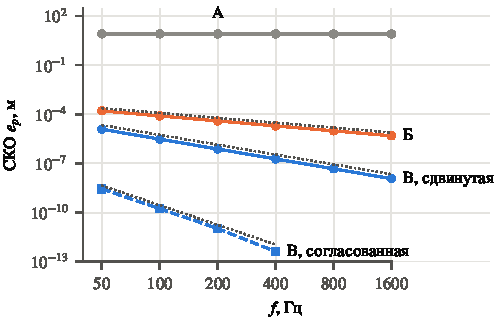
\includegraphics[width=\columnwidth]{figures/convergence.pdf}
  \caption{СКО ошибки положения при обратном интегрировании схемой РК4. Пунктир~--- наклоны $h^1$, $h^2$, $h^4$; для модели В на согласованной сетке при $f>400$~Гц ошибка ограничена округлением (около $10^{-12}$~м) и не показана.}
  \label{fig:conv}
\end{figure}

Схема первого порядка~\eqref{eq:integr} не различает модели Б и В: её собственная ошибка (около 10~см) больше различия между ними. РК4 различает их. На сдвинутой сетке при 200~Гц ошибка модели Б в 50 раз больше, чем у модели В, и разрыв растёт с частотой. На согласованной сетке модель Б даёт первый порядок из-за выбора значения в узле (подраздел~IV-F). С односторонним пределом слева в конце шага порядок поднимается до 3,8, но реальный датчик выдаёт в каждый момент одно значение, поэтому практически значим результат на сдвинутой сетке. Модель А не согласована с движением: ошибка около 8~м не зависит от $h$.

Наблюдаемые порядки на сдвинутой сетке совпадают с оценкой $\min(4,m+1)$ (табл.~\ref{tab:orders}), в том числе для ориентации. Ошибка ориентации при 200~Гц: $4{,}0\cdot10^{-8}$~рад для модели Б и $5{,}7\cdot10^{-11}$~рад для модели В. Для модели А, где показания содержат $\delta$-импульсы, номер $m$ не определён, и оценка к ней не применима; порядок 4 на согласованной сетке тоже получается не из неё, а потому, что узлы не попадают внутрь шага.

\begin{table}[!tb]
  \caption{Порядок сходимости РК4 на сдвинутой сетке}
  \label{tab:orders}
  \centering
  \small
  \begin{tabular}{llcccc}
    \toprule
    Ошибка & Модель & Разрывна & $m$ & $\min(4,m+1)$ & Получено \\
    \midrule
    $e_p$ & Б & $\vb a_B$ & 0 & 1 & 1,01 \\
    $e_p$ & В & $\dot{\vb a}_B$ & 1 & 2 & 2,00 \\
    $e_R$ & Б & $\dot{\boldsymbol\omega}_B$ & 1 & 2 & 2,00 \\
    $e_R$ & В & $\ddot{\boldsymbol\omega}_B$ & 2 & 3 & 3,00 \\
    \bottomrule
  \end{tabular}
\end{table}

\subsection{Шумовая часть генератора}

Для серии~2 сгенерирована трёхчасовая запись неподвижного датчика с частотой 200~Гц и тестовыми интенсивностями порядка типичных MEMS-датчиков: $\sigma_g=1{,}7\cdot10^{-4}$~рад/(с$\cdot\sqrt{\text{Гц}}$), $\sigma_{bg}=2{,}0\cdot10^{-5}$~рад/(с$^2\cdot\sqrt{\text{Гц}}$), $\sigma_a=2{,}0\cdot10^{-3}$~м/(с$^2\cdot\sqrt{\text{Гц}}$), $\sigma_{ba}=3{,}0\cdot10^{-3}$~м/(с$^3\cdot\sqrt{\text{Гц}}$). По вариации Аллана интенсивности белого шума восстановлены по всем осям с отклонением не более 0,7\%, интенсивности случайного блуждания~--- не более 6\% (гироскоп~--- 4\%). Больший разброс для случайного блуждания объясняется тем, что оно определяется по большим $\tau$, где число независимых интервалов мало.

% ============================================================
\section{Заключение}

Формализовано необходимое и достаточное условие непрерывности идеальных показаний IMU при произвольной внешней калибровке: положение и ориентация камеры должны принадлежать классу $C^2$. Для модели на B-сплайнах приведены замкнутые выражения угловой скорости и углового ускорения и доказана гладкость на стыках отрезков. Сформулированы задачи построения траектории, генерации и проверки и исследована их корректность.

Вычислительный эксперимент подтвердил выводы. Кусочно-линейная модель со SLERP не согласована с движением (ошибка около 8~м за 10~с при любой частоте). Модель со SQUAD даёт скачки углового ускорения и, через рычаг, показаний акселерометра; порядок сходимости по положению падает до первого. Модель на B-сплайнах даёт по положению порядок 2 на сдвинутой и 4 на согласованной сетке. На сдвинутой сетке наблюдаемый порядок совпал с оценкой $\min(4,m+1)$ во всех проверенных случаях и может служить численной мерой гладкости модели движения. Задача построения ориентации с условиями на угловую скорость на концах решена методом Левенберга--Марквардта до машинной точности. Шумовая часть генератора воспроизводит заданные интенсивности. Влияние шума и дрейфа на точность восстановления и проверка на реальных VIO-алгоритмах~--- предмет дальнейшей работы.

Модель кинематическая (Д6). Для квадрокоптера ориентация и ускорение связаны через направление тяги, поэтому независимое задание $\vb p(t)$ и $R(t)$ может давать движения, недостижимые для реального аппарата. Развитием работы является генерация траекторий с учётом динамики носителя, например методом минимального снэпа~\cite{mellinger}, где требуется гладкость положения выше $C^2$.

% ============================================================
\begin{thebibliography}{99}

\bibitem{vinsmono} Qin T., Li P., Shen S. VINS-Mono: A Robust and Versatile Monocular Visual-Inertial State Estimator // IEEE Transactions on Robotics. 2018. Vol.~34, No.~4. P.~1004--1020.

\bibitem{orbslam3} Campos C., Elvira R., Gómez Rodríguez J.J., Montiel J.M.M., Tardós J.D. ORB-SLAM3: An Accurate Open-Source Library for Visual, Visual-Inertial, and Multimap SLAM // IEEE Transactions on Robotics. 2021. Vol.~37, No.~6. P.~1874--1890.

\bibitem{openvins} Geneva P., Eckenhoff K., Lee W., Yang Y., Huang G. OpenVINS: A Research Platform for Visual-Inertial Estimation // 2020 IEEE International Conference on Robotics and Automation (ICRA). Paris, 2020. P.~4666--4672.

\bibitem{euroc} Burri M., Nikolic J., Gohl P., Schneider T., Rehder J., Omari S., Achtelik M.W., Siegwart R. The EuRoC Micro Aerial Vehicle Datasets // The International Journal of Robotics Research. 2016. Vol.~35, No.~10. P.~1157--1163.

\bibitem{tumvi} Schubert D., Goll T., Demmel N., Usenko V., Stückler J., Cremers D. The TUM VI Benchmark for Evaluating Visual-Inertial Odometry // 2018 IEEE/RSJ International Conference on Intelligent Robots and Systems (IROS). Madrid, 2018. P.~1680--1687.

\bibitem{woodman} Woodman O.J. An Introduction to Inertial Navigation: Technical Report UCAM-CL-TR-696. Cambridge: University of Cambridge, Computer Laboratory, 2007.

\bibitem{shoemake} Shoemake K. Animating Rotation with Quaternion Curves // ACM SIGGRAPH Computer Graphics. 1985. Vol.~19, No.~3. P.~245--254.

\bibitem{kerbl} Kerbl B., Kopanas G., Leimkühler T., Drettakis G. 3D Gaussian Splatting for Real-Time Radiance Field Rendering // ACM Transactions on Graphics. 2023. Vol.~42, No.~4. Art.~139.

\bibitem{sturm} Sturm J., Engelhard N., Endres F., Burgard W., Cremers D. A Benchmark for the Evaluation of RGB-D SLAM Systems // 2012 IEEE/RSJ International Conference on Intelligent Robots and Systems (IROS). Vilamoura, 2012. P.~573--580.

\bibitem{zhang} Zhang Z., Scaramuzza D. A Tutorial on Quantitative Trajectory Evaluation for Visual(-Inertial) Odometry // 2018 IEEE/RSJ International Conference on Intelligent Robots and Systems (IROS). Madrid, 2018. P.~7244--7251.

\bibitem{epifanov} Епифанов К.А. Исследование алгоритмов замыкания цикла в лидарной одометрии // Искусственный интеллект в промышленных, коммерческих, медицинских и финансовых приложениях: сб. ст. науч.-техн. семинара. Вып.~3 / под ред. А.Р.~Ефимова. М.: НИТУ «МИСИС», 2025. С.~57--61.

\bibitem{ermolenko} Ермоленко И.Д. Анализ эффективности методов стереозрения для восстановления 3D-облака точек по карте диспаритета // Искусственный интеллект в промышленных, коммерческих, медицинских и финансовых приложениях: сб. ст. науч.-техн. семинара. М.: НИТУ «МИСИС», 2026. С.~34.

\bibitem{furgale} Furgale P., Rehder J., Siegwart R. Unified Temporal and Spatial Calibration for Multi-Sensor Systems // 2013 IEEE/RSJ International Conference on Intelligent Robots and Systems (IROS). Tokyo, 2013. P.~1280--1286.

\bibitem{lovegrove} Lovegrove S., Patron-Perez A., Sibley G. Spline Fusion: A Continuous-Time Representation for Visual-Inertial Fusion with Application to Rolling Shutter Cameras // Proceedings of the British Machine Vision Conference (BMVC). Bristol, 2013.

\bibitem{patronperez} Patron-Perez A., Lovegrove S., Sibley G. A Spline-Based Trajectory Representation for Sensor Fusion and Rolling Shutter Cameras // International Journal of Computer Vision. 2015. Vol.~113, No.~3. P.~208--219. DOI: 10.1007/s11263-015-0811-3.

\bibitem{kim} Kim M.-J., Kim M.-S., Shin S.Y. A General Construction Scheme for Unit Quaternion Curves with Simple High Order Derivatives // Proceedings of the 22nd Annual Conference on Computer Graphics and Interactive Techniques (SIGGRAPH~'95). 1995. P.~369--376.

\bibitem{mueggler} Mueggler E., Gallego G., Rebecq H., Scaramuzza D. Continuous-Time Visual-Inertial Odometry for Event Cameras // IEEE Transactions on Robotics. 2018. Vol.~34, No.~6. P.~1425--1440.

\bibitem{sommer} Sommer C., Usenko V., Schubert D., Demmel N., Cremers D. Efficient Derivative Computation for Cumulative B-Splines on Lie Groups // Proceedings of the IEEE/CVF Conference on Computer Vision and Pattern Recognition (CVPR). 2020. P.~11145--11153. DOI: 10.1109/CVPR42600.2020.01116.

\bibitem{haarbach} Haarbach A., Birdal T., Ilic S. Survey of Higher Order Rigid Body Motion Interpolation Methods for Keyframe Animation and Continuous-Time Trajectory Estimation // 2018 International Conference on 3D Vision (3DV). Verona, 2018.

\bibitem{imusim} Young A.D., Ling M.J., Arvind D.K. IMUSim: A Simulation Environment for Inertial Sensing Algorithm Design and Evaluation // Proceedings of the 10th International Conference on Information Processing in Sensor Networks (IPSN). Chicago, 2011. P.~199--210.

\bibitem{ovcode} OpenVINS: исходный код класса BsplineSE3 (файл ov\_core/src/sim/BsplineSE3.h) [Электронный ресурс]. URL: \url{https://github.com/rpng/open_vins/blob/master/ov_core/src/sim/BsplineSE3.h} (дата обращения: 19.11.2026).

\bibitem{shoemake87} Shoemake K. Quaternion Calculus and Fast Animation // SIGGRAPH 1987 Course Notes \#10: Computer Animation: 3-D Motion Specification and Control. 1987. P.~101--121.

\bibitem{ly} Ly K.T., Semenov V., Risiglione M., Merkt W., Havoutis I. R-LGP: A Reachability-guided Logic-geometric Programming Framework for Optimal Task and Motion Planning on Mobile Manipulators // 2024 IEEE International Conference on Robotics and Automation (ICRA). Yokohama, 2024. P.~14917--14923. DOI: 10.1109/ICRA57147.2024.10611389.

\bibitem{sola} Solà J. Quaternion Kinematics for the Error-State Kalman Filter // arXiv preprint arXiv:1711.02508. 2017.

\bibitem{forster} Forster C., Carlone L., Dellaert F., Scaramuzza D. On-Manifold Preintegration for Real-Time Visual-Inertial Odometry // IEEE Transactions on Robotics. 2017. Vol.~33, No.~1. P.~1--21.

\bibitem{ieee952} IEEE Std 952-1997. IEEE Standard Specification Format Guide and Test Procedure for Single-Axis Interferometric Fiber Optic Gyros. New York: IEEE, 1998. DOI: 10.1109/IEEESTD.1998.86153.

\bibitem{deboor} Де Бор К. Практическое руководство по сплайнам / пер. с англ. М.: Радио и связь, 1985. 303~с.

\bibitem{kim95} Kim M.-J., Kim M.-S., Shin S.Y. A C$^2$-Continuous B-spline Quaternion Curve Interpolating a Given Sequence of Solid Orientations // Proceedings of Computer Animation~'95. 1995. P.~72--81.

\bibitem{mellinger} Mellinger D., Kumar V. Minimum Snap Trajectory Generation and Control for Quadrotors // 2011 IEEE International Conference on Robotics and Automation (ICRA). Shanghai, 2011. P.~2520--2525.

\end{thebibliography}

\end{document}
